% This is LLNCS.DOC the documentation file of
% the LaTeX2e class from Springer-Verlag
% for Lecture Notes in Computer Science, version 2.4
\documentclass{llncs}
\usepackage{llncsdoc}
\usepackage{graphicx} 
%
\begin{document}
\thispagestyle{empty}
\rule{\textwidth}{1pt}
\vspace{2pt}
\begin{flushright}
\Huge
\begin{tabular}{@{}l}
Barriers to the\\
implementation of\\
k-anonymity and\\
related microdata\\
anonymization techniques\\
in a realworld application\\[6pt]

\end{tabular}
\end{flushright}
\rule{\textwidth}{1pt}
\vfill
\title{Barriers to the implementation of k-anonymity and related microdata anonymization techniques in a realworld application}
\author{Andreas Wiegnand, 1878334\\
	Ludwig Schallner, 1850413}
\institute{}
\maketitle
%
\newpage
\section{Introduction}
%
Nowadays data is a key factor in every domain. Some compare it with the gold rush of
The 19. Century\cite{datarevo}. But to use the data for commercial or scientific purposes the privacy of the dataholder does not have to be compromised.\\

The so called k-anonymity method, is theoretical a good one to make anonymous data but there are practical barriers that will occur in the real world. Those prevent such implementation. The goal of k-anonymity is, to prevent the possibility to get information about the real individual, or at least with k other possible individuals \cite{sweeney2002k}. So if a individual is discriped by a tuple of \ensuremath{\langle f_1, ... ,f_n \rangle} features and each feature can have \ensuremath{\langle a_1,...,a_n \rangle} attributes \cite{sweeney2002k}. There are at least k other individual with the same attribute for each feature so that there is no possibility to reduce the real individual and there will be at least k individuals with the same tuple\cite{sweeney2002k}. The attributes that are used to link the external data is called quasi identifiers. Typical values for them are gender, date of birth and zip code \cite{ldiversity}. \\

We will present techniques that override k-anonymity and get the real individual. Another problem we will introduce is, that the producing of k-anonymity of a computational view is a NP-hard problem, like  meyersond and williams shown.
...
%\\\\WAS IST DAS HIER
%Sets of attributes (like gender, date of birth, and zip code
%in the example above) that can be linked with external data
%to uniquely identify individuals in the population are called
%quasi-identifiers.
%Attributes that clearly
%identify individuals. These are known as explicit identifiers
%and include Social Security Number, Address, and Name,
%and so on.\cite{li2007t}.
\section{Basics}
The definiton of microdata should be clear, therefore in the following on what 
\section{Barriers against K-anonymity}
\begin{enumerate}
	\item Producing k-anonymity
	\item Reidentify dataholders by linking or matching the data to the data or by looking at unigque characterstics found the the released data.
\end{enumerate}
\cite{maheshwarkar2011privacy}
\subsection{Linking data}

Another problem to do the implementation of k-anonymity, the attacker can take another dataset and link both together to get rid off the k-anonymity and infer the real individual. This process is called linking data and was first described by Sweeney\cite{sweeney2002k}. She showed that with a example of health care data from 37 states in the USA. The institute from which she bought the data, insures the anonymity of the individuals. Sweeney purchased the voter registration list for Cambridge Massachusettts and received information of the voters including ZIP code, birth date and gender of each voter.She linked that information with the medical data. It was possible to deanonymize the data  and get ethnicity, visit date, diagnosis, procedure, medication and total charge of some patients \cite{sweeney2002k}. 
\\
\begin{figure}[]
	\centering
	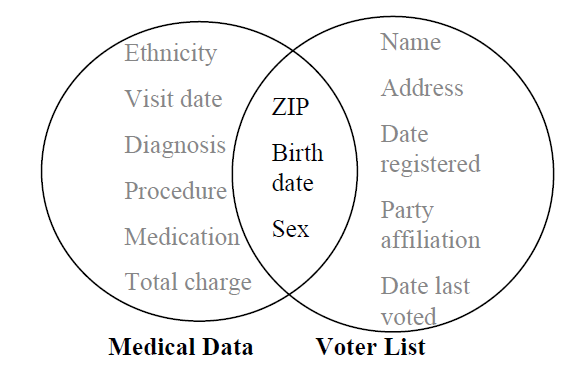
\includegraphics[width=0.7\textwidth]{linkingdata.png}
	\caption{linking data}%
\end{figure}

You got 2 datasets A and B. Each dataset got \ensuremath{\langle f_1, ... ,f_n \rangle} features and \ensuremath{\langle r_1, ... ,r_n \rangle} rows.
Each row is then a tuple \ensuremath{r_i} with n features \ensuremath{\langle f_1, ... ,f_n \rangle} describing the individual.
And A got k-anonimity you can get rid oft he anonymity of the individual by linking the A to B. So if \ensuremath{A \cap B \not \neq \emptyset} it is possible to infer the anonymized individual \cite{sweeney2002k}.
\\ ...
% Please add the following required packages to your document preamble:
% \usepackage{longtable}
% Note: It may be necessary to compile the document several times to get a multi-page table to line up properly
\subsection{Unsorted matching attack against k-anonymity}

There is a possibility of a leak of information, if the release k-anonymity data is in some kind of a sort release. This mean the numerical attributes are descending or ascending sorted and attributes, which be of characters are alphabetical ordered, can give the attacker Information about the sensitive data. To prevent this attack, just get the data into a random order with a pseudo randomized sorting algorithm \cite{sweeney2002k}. As an example take a look at the table 3: matching attack  will give an example on that. If you compare the different release generalized tables you can figure out all quasi identifier of those \cite{sweeney2002k}.
\\...
\begin{table}	
	\caption{matching attack}
	\centering
	\begin{tabular}[t]{|l|l|}		
	\hline
	Age & ZIP   \\ \hline
	2   & 91058 \\ 
	4   & 91058 \\ 
	50  & 27785 \\ 
	52  & 27785 \\ 
	20  & 32105 \\ 
	21  & 32105 \\ 
	31  & 67676 \\ 
	32  & 67676 \\ \hline
		\end{tabular}
	\hfill
	\begin{tabular}[t]{|l|l|}
	\hline
	Age & ZIP   \\ \hline
	*   & 91058 \\
	**   & 91058 \\
	5*  & 27785 \\
	5*  & 27785 \\
	2*  & 32105 \\
	2*  & 32105 \\
	3*  & 67676 \\
	3*  & 67676 \\ \hline  
	\end{tabular}
	\hfill
	\begin{tabular}[t]{|l|l|}
	\hline
	Age & ZIP   \\	\hline
	2   & 91*   \\
	4   & 91*   \\
	50  & 27*   \\
	52  & 27*   \\
	20  & 32*   \\
	21  & 32*   \\
	31  & 67*   \\
	32  & 67*   \\ \hline  
	\end{tabular}
\end{table}
\subsection{Complementary release attack against k-anonymity}

The problem of complementary release attack against k-anonymitym lies by the release of other k-anoymitizet tables from the same dataset. To stop the attack the data holder should consider for each release of data if it's possible to release information with older released data. This is hard to avoid especially when the data can come from different individuals \cite{sweeney2002k}.
\\...
\subsection{Temporal attack against k-anonymity}

The data can be change over time. New tuples might be added or persistent ones can be changed. If the GT0 was release at time T=0 and on a later time GT1 will be released at time T = 1 with new tuples of information. Both tables at their time stamp T are k-anonymity, but it will not be checked if they are k-anonymity between them. So their is a possibility of information leaking and a failure oft he k-anonymity in both tables \cite{sweeney2002k}.
\\...
\subsection{Homogeneity Attack}
%Alice and Bob are antagonistic neighbors. One day Bob falls ill and is taken by ambulance to the hospital. Having seen the ambulance, Alice sets out to discover what disease Bob is suffering from. Alice discovers the 4-anonymous table of current inpatient records published by the hospital \textbf{(Figure 2}), and so she knows that one of the records in this table contains Bob?s data. Since Alice is Bob's neighbor, she knows that Bob is a 31-year-old American male who lives in the zip code 13053.  Therefore, Alice knows that Bob?s record number is 9,10,11, or 12.\\Now, all of those patients have the same medical condition (cancer), and so Alice concludes that Bob has cancer. \textbf{Observation 1} k-Anonymity can create groups that leak information due to lack of diversity in the sensitive attribute. Note that such a situation is not uncommon. As a back-of-the-envelope calculation, suppose we have a dataset containing 60,000 distinct tuples where the sensitive attribute can take 3 distinct values and is not correlated with the nonsensitive attributes. A 5-anonmyization of this table will have around 12,000 groups2 and, on average, 1 out of every 81 groups will have no diversity (the values for the sensitive attribute will all be the same). Thus we should expect about 148 groups with no diversity. Therefore, information about 740 people would be compromised by a homogeneity[11] attack. This suggests that in addition to k-anonymity, the sanitized table should also ensure ?diversity? ? all tuples that share the same values of their quasi-identifiers should have diverse values for their sensitive attributes.Our next observation is that an adversary could use?background? knowledge to discover sensitive information. Homogeneity attack applies on the non diversity of sensitive data. If the attack knows the quasi idenfifier and because oft he k-anonymity. He will get back 8 possible users. But all oft hem got the same senstive Data attribute. The attack knows now the sensitive data of his victim.[11]

\subsection{Background Knowledge Attack}

Taking background knowledge attack from a person and take it into account to derive the sensitive data. In our example of table 1 this could be that we know one person my name, age, and nationality. Additionally we know, because that she is asian, in would be unusual that she got diabetes, because diabetes is a uncommon sickness in japan \cite{ldiversity}.
\\...
\subsection{Complexity of producing k-anonymity}
Till now we only looked at problems of information leaking and privacy problems for individuals. Data is personal-specific information which is structured as a table in rows and columns. Rows a tuple. The columns are attributes with are a set of values which describe the certain attribute. A tuple specify a person. K-anonymity is about protecting the identity of a person not relationships of companies or governments. So the goal of k-anonymity is, not getting more information by linking the data to external data. The bridge between the data and external data is called "quasi-identifier". Examples for that would be ZIP, gender, birth date etc.. \\
\\
Generalization mean, replacing a value with a less specific but semantic identical value. For example we got a list of forenames of buys, (Achmed, Achilles, Achim). To generalize this names you can just (Ach*,Ach*, Ach*) delete the last chars of the name. So there is a less specific domain and now more generalize through this mapping. Suppression on the other hand means not releasing the value at all.
\\...
%In this section we presented formal notions of: (1) generalization incorporating suppression; (2) minimal generalization; and, (3) minimal distortion
%\section{Methods}
%Unless otherwise stated, the term data refers to person-specific information that is conceptually organized as a table of rows (or records) and columns (or fields). Each row is termed a tuple. Which contains a relationship among the set of values associated with a person. Disclosure means that explicit or inferable information about a person was released that was not intended .
\subsection{L-Diversity}

K-anonymity gives protection on the identity disclosure. L-Diversity more with the same sensitive data. 
\subsubsection{Skewness Attack} 
When the overall distribution is skewed, satisfying l-diversity does not prevent attribute disclosure.  Now consider an equivalence class that has 49 positive Records and only one negative record. It would be distinct 2-diverse and has higher entropy than the overall table (and thus satisfies any entropy l-diversity that one can impose), even though anyone in the equivalence class would be considered 98\% positive, rather than 1\% percent. In fact, this equivalence class has exactly the same diversity as a class that has one positive and 49 negative records, even though the two classes present very different levels of privacy risks \cite{ldiversity}. 
\\...
\subsubsection{Similarity Attack} 
When the sensitive attribute values in an equivalence class are distinct but semantically similar, an adversary can learn important information [8]. Positive and negative disclosure: the homogeneity attack where A determined that B has cancer is an example of positive disclosure, whereas when an adversary eliminates some possibilities of sensitive tuples is known as negative disclosure. This negative disclosure uses background knowledge attack. L-diversity also fails in the case of multiple sensitive attributes. In short, distributions that have the same level of diversity may provide very different levels of privacy, because there are semantic relationships among the attribute values. Furthermore different values have very different levels of sensitivity, and  privacy is also affected by the relationship with the overall distribution. l-diversity does not consider semantic meanings of sensitive values. l-diversity cannot provide privacy for the multiple sensitive attributes \cite{ldiversity}.
\\...
\subsection{t-Closeness}
The publication of Ninghui, Tiancheng and Suresh is about the t-closeness, which takes into account the unavoidable gain of knowledge of an attacker (the weakness of $\ell$-diversity) \cite{li2007t}. To archive t-closeness a special distance measurement method the Earth Mover's Distanz (EMD) is used \cite{rubner2000earth}. Furthermore t-closeness "requires that the distribution of a sensitive attribute in any equivalence class is close to the distribution of the attribute in the overall table" \cite{li2007t}.\\
 
The weakness of t-closeness by using EMD is that it does not takes the into account if a change of pairs is more significant than another one, which an attacker can use \cite{li2007t}. A combination of EMD and Kullback-Leibler Distance \cite{kullback1951} will help to prevent this attack \cite{li2007t}.
\\

The distribution of the sensitive data in the table is the same like the real data\cite{li2007t}. The t-closeness principle: An equivalence class is said to have t-closeness if the distance between the distribution of a sensitive attribute in this class and the distribution of the attribute in the whole table is no more than a threshold t. A table is said to have t-closeness if all equivalence classes have t-closeness\cite{li2007t}.
...
\begin{figure}[h]
	\centering
	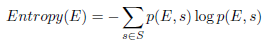
\includegraphics[width=0.7\textwidth]{entropy.png}
	\caption{Definition of a entropy of an equivalence class E}%
\end{figure}
\newpage
\bibliography{literature}
\bibliographystyle{splncs03}
\end{document}
